\documentclass[]{report}

\setcounter{secnumdepth}{0}
\usepackage[margin=1in]{geometry}
\usepackage{caption}
\usepackage{parskip}
\usepackage{float}
\usepackage{graphicx}
\usepackage{subcaption}
\usepackage[section]{placeins}
\newfloat{Equation}{H}{lop}
\usepackage[backend=biber, style=authoryear]{biblatex}
\addbibresource{./report.bib}

\title{
	The Relative Neuroplasticity of Artificial
	\linebreak
	and Biological Neural Network Configurations
}
\author{Oliver Balfour}

\date{%
	Alfred Deakin High School\\[2ex]%
	\today
}

\begin{document}
\maketitle

\begin{abstract}
	In this experiment the neuroplasticity of neural networks, both artificial and biological, was tested. Several configurations of computing machines, ranging from simple dense feed-forward Multi-Layer Perceptrons (MLPs) and Artificial Neural Networks (ANNs) to more complex Recurrent Neural Networks (RNNs), were tested, with the human brain as a baseline for performance. Also tested was a Support Vector Machine (SVM), a much older algorithm with a mathematical and not biologically-inspired approach to classification, to gauge how far the field of Machine Learning has come in the past decades both in terms of performance and neuroplasticity. Each machine was tested (with minor programmatic alterations to the input and output layers of each artificial model to account for differing input sizes) against several different classification and regression problems including but not limited to classifying handwritten digits (using the MNIST dataset) and performing sentiment analysis on highly polarized movie reviews (using the SAR14 IMDb review dataset). The neuroplasticity of each model was then evaluated based on the standard deviation of the error rates of each model in each of the problems tested.
\end{abstract}

\tableofcontents
\newpage

\section{Introduction}

The human brain is capable of rewiring itself throughout its lifetime (\cite{draganski2004neuroplasticity}). This feature, known as neuroplasticity, is the driving force behind the process of learning, and is present in a wide range of animals. It was first discovered in rats in the 1960s (\cite{bennett1964chemical}), and the theory behind it has applications as far as artificial intelligence and machine learning. In this experiment, the extent to which various configurations of Artificial Neural Networks (ANNs) exhibit neuroplasticity is tested, by teaching the same ANNs to perform very diverse tasks, compared to a baseline of the performance of the human brain.

The aim of this experiment is to determine how far behind in terms of neuroplasticity modern Artificial Neural Networks (ANNs) are when compared with the human brain. This is done by training the same artificial and biological neural network configurations to perform several different classification and regression tasks, and measuring the standard deviation of the error rates across each problem as a measure of neuroplasticity.

It is hypothesised that:
\begin{enumerate}
	\item The human brain will marginally surpass state-of-the-art ANN configurations in all problem domains, and will perform exceptionally well in all problem domains. (Refer to the method on page \pageref{itm:Method} for a full list of problems tested.)
	\item The Recurrent Neural Network (RNN) will perform well on all problems, but particularly the sentiment analysis problem.
	\item The standard densely-layered feed-forward Artificial Neural Network (ANN) will perform acceptably on all problems.
	\item The Support Vector Machine (SVM) will perform well recognising handwritten digits and classifying iris genuses, but will perform sub-par in all other problem domains.
\end{enumerate}

\section{Literature Review}

Whilst there is plenty of literature on machine learning and neuroplasticity as separate topics, there is very little directly relating to both. The only publicly available scientific paper pertaining to both merely documents a method for making an ANN neuroplastic (\cite{perwej12}), however its approach is essentially a synaptic pruning method for reducing overfitting in ANNs similar to the well-established method of neural network dropout, which randomly discards nodes from a neural network to reduce overfitting (\cite{dropout14}). The only other paper referring to both topics is behind an expensive journal paywall.

This experiment focuses on a neglected area within the field of machine learning: as artificial intelligence research is primarily focused on highly specialised cutting-edge techniques, investigation into the re-usability and adaptivity of neural networks has been left behind. Considering that a true artificial intelligence requires an extremely plastic brain to be capable of learning without requiring a considerable number of nested neural networks for each individual task it is capable of performing, this investigation is important as a measure of the level of progress that the field of machine learning has achieved toward an Artificial General Intelligence (AGI), not in terms of specialised narrow intelligence feats such as those of AIs designed solely to play games like Chess or Go at a highly competitive level, but in terms of how specialised narrow AI achievements can be generalised, or bridged across to one another to create a neuroplastic general intelligence.

The techniques used to create neural networks in this experiment, however, are very well documented. The perceptron, an outdated artificial model of a neuron, was documented thoroughly by its creator (\cite{rosenblatt1958perceptron}), the multi-layer perceptron model, an improved model that featured hidden layers and the backpropagation algorithm was documented in a well established journal (\cite{rumelhart1986learning}); likewise, the original Support Vector Machine algorithm was well documented (\cite{vapnik1995support}). All of the neural network configurations used in this experiment rely on well-established methods that have been hot topics in the world of AI research over the past few decades. Simple feed-forward backpropagated sigmoid ANNs have been in wide use since the late 1980s, and CNNs and RNNs were both designed as more specialised improvements on the simpler ANN and MLP structures.

\section{Background Information}

A neural network is essentially a simplified computer abstraction of a brain, with primitive and computationally inexpensive representations of the core functions of neurons in a real life brain. Neural networks are organised into layers, usually at least three, which contain distinct neurons. The first layer takes binary or floating-point input from the host computer program, and the last returns binary output back to the host program. In feed-forward neural networks, the most common type of neural network, simulated signals pass forward through neurons layer by layer without any form of recursion.

\begin{figure}[H]
	\centering
	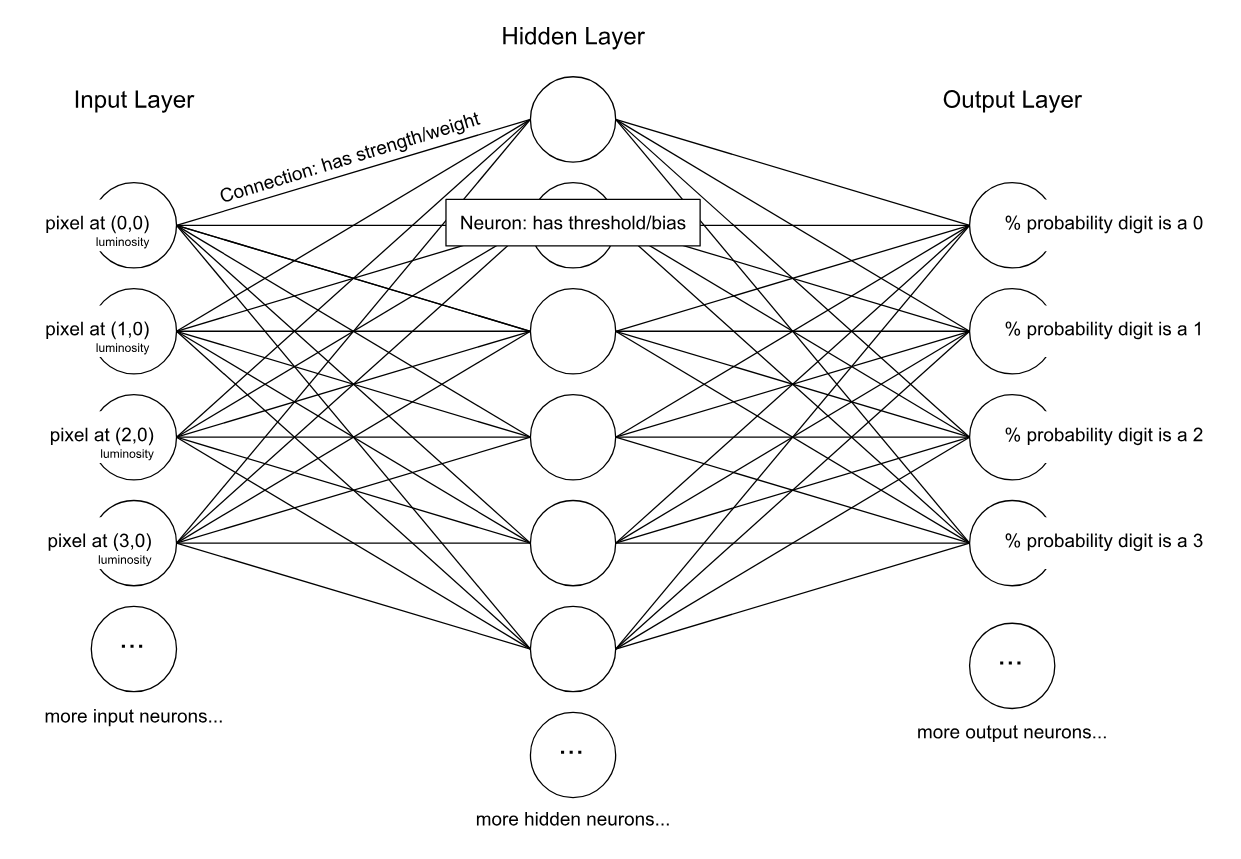
\includegraphics[width=0.8\textwidth]{network.png}
	\caption{Diagram of a feed-forward Artificial Neural Network trained to recognise digits.}
	\label{fig:network}
\end{figure}

A neuron is typically represented by a series of numbers: an activation threshold (bias), and a series of numbers representing the strengths of connections with neurons in the previous layer. Given the outputs (activations) of the neurons in the previous layer (or given the input data from the host program in the case of the input layer), a neuron's output (activation) will equal the sum of all of previous layer's neurons activations multiplied by the connection strengths (weights), with the activation threshold (bias) of the neuron in question being subtracted. In a more traditional perceptron model, the output would be transformed such that if it is positive it is a binary 1, and if it is negative it is a binary 0; however more modern sigmoid models usually transform this value into a floating-point decimal between 0 and 1 using a learning function.

In this experiment, both perceptron and sigmoid neurons are tested, as well as a Support Vector Machine (SVM), which is an older algorithm designed for classification problems.

\begin{Equation}
	\begin{equation}
		n_a = \left\{ \begin{array}{ll}
		0 & \mbox{if } \sum_i M_{i_a} M_{i_w} \leq n_b \\
		1 & \mbox{if } \sum_i M_{i_a} M_{i_w} > n_b
		\end{array}\right.
	\end{equation}
	\caption{Activation (output value) of a perceptron.}
\end{Equation}

\begin{Equation}
	\begin{equation}
		n_a = \sum_{i=0}^{|M|}(M_{i_a} M_{i_w}) - n_b
	\end{equation}
	\caption{Activation of an artificial sigmoid neuron, before applying a learning function.}
\end{Equation}

In the above equations, \(M\) is the set of neurons from the previous layer, \(M_{i_w}\) is the weight (or axon-dendrite connection strength) of the \emph{i}th neuron, and \(M_{i_a}\) denotes the activation (output value, a floating-point number from 0 to 1 transformed by a learning function); \(n\) is the neuron whose output is being calculated and \(n_b\) its bias (activation/firing threshold.)so the above formula boils down to adding all of the connection weights multiplied by the outputs, and then subtracting the bias. In the sigmoid model, a negative value means the neuron does not fire, as the threshold has not been reached, and a positive the opposite. The output is wrapped in a function to make the output smoother and more efficient at learning, but that is an irrelevant implementation detail. In the perceptron model, a negative value is replaced with a 0 and a positive with a 1.

The weights and biases of each neuron and neuronal connection are optimised to serve a specific purpose through the process of training. Usually, these values will start as random numbers, and through a process known as Stochastic Gradient Descent the values are slowly optimised until the neural network model is sufficiently good at its task. (Refer to the glossary on page \pageref{itm:SGD} for more information on Stochastic Gradient Descent.) There are many applications for neural networks: A neural network may be trained to classify images (computer vision and optical character recognition), to estimate data such as house or stock prices given data about their respective markets, or even to control robots. This adaptivity, or neuroplasticity, is investigated in this report.

Nodes in neural networks are quite similar to their biological counterparts, in that they have a constant activation threshold (in biological neurons this threshold is -55mV, whereas in artificial sigmoid neurons this is a unique number which is recursively optimised during the training process), take input from other neurons they have connections with (although sigmoid neurons have differing connection strengths and are connected to all nodes in the previous layer; biological neurons simply have binary connection strenghts --- they either are or are not connected), and produce one output which is used as an input by additional nodes in the network. The primary difference between neural networks and brains overall is that brains, even in rodents and insects, have many orders of magnitude more neurons, and learning algorithms in biological networks are the fine-tuned result of billions of years of evolutionary processes.

\label{itm:Method}
\section{Method}

There are 6 neural networks tested in this experiment, against 4 different classification and regression problems, each in different problem domains. The neural network configurations are listed below:

\begin{enumerate}
	\item A Support Vector Machine (SVM), to show the inefficiency of traditional mathematical or logical approaches compared to biologically inspired.
	\item 8 different densely-layered feed-forward Multi-Layer Perceptrons (MLPs) using perceptrons instead of sigmoid neurons (2 sets of 4 different models with differing hidden layer configurations, one set with dropout and one without).
	\newline
	The 4 hidden layer configurations are:
	\begin{enumerate}
		\item 1 hidden layer with 32 neurons
		\item 1 hidden layer with 256 neurons
		\item 2 hidden layers with 256 neurons each
		\item 2 hidden layers with 512 neurons each
	\end{enumerate}
	All dropout-enabled models have the dropout percentage set to 20\% (so 20\% of neurons are randomly discarded throughout the learning process.)
	\item 8 standard densely-layered feed-forward sigmoid Artificial Neural Networks (ANNs), with hidden layer configurations identical to those of the MLPs above, aside from the nonbinary activation function.
	\item 4 Recurrent Neural Networks (RNNs), with 1 Long Short-Term Memory (LSTM) hidden layer containing 32 or 128 neurons. Two models have dropout, the others do not.
	\newline
	The recurrent neural networks use RMSprop (\cite{hinton2012neural}) instead of SGD as a learning algorithm, as it has been recorded to perform better with RNNs.
	\item And as a baseline for performance and neuroplasticity, several people are used.
\end{enumerate}

It was decided that Convolutional Neural Networks (CNNs) should not be included in the experiment, as although they are a very popular type of neural network, they only work with multidimensional spatial or temporal data (their primary use-cases are in computer vision, optical character recognition, and audio analysis.) This means that they cannot feasibly compute linear regression or non-temporal classification functions without having their kernel layers configured to apply no transformation to the data (by having nil values for all cells except the centre, which would have a 1, such that each kernel operation merely acts as a cat operation.)

Each of the above models will be tested against the following classification and regression problems:

\begin{enumerate}
	\item Handwritten digit recognition (using the MNIST dataset)\footnote{The MNIST dataset is available at: http://yann.lecun.com/exdb/mnist/}
	\item Iris flower classification (using Fisher's dataset\footnote{The Iris dataset is available at: http://archive.ics.uci.edu/ml/datasets/Iris} (\cite{uciml2007}))
	\item Sentiment analysis (using the Large Movie Review Dataset of IMDb movie reviews (\cite{maas2011imdb}))
	\item Breast cancer diagnosis (using the University of Wisconsin dataset\footnote{The Breast Cancer diagnosis dataset is available at: http://archive.ics.uci.edu/ml/datasets/Breast+Cancer+Wisconsin+(Diagnostic)})
\end{enumerate}

The human brain will be tested against each of the aforementioned problems, although due to the varying nature and medium in which the datasets above are presented in, which means different cortices of the human brain will be used for different problem domains, the human test subjects will have a not insignificant advantage over their machine counterparts.

To avoid allowing the human test subjects to utilise areas of their brains which have already been trained in the problem domains this experiment is testing (such as allowing a native English speaker perform the sentiment analysis problem on polarised English movie reviews), all of the textual samples have been machine-translated (using Google Translate) into Korean, a lanuage with a different semantic structure, which does not share any major linguistic roots, and which is reliably machine-translated. Additionally, in the digit recognition problem, all images of handwritten digits are transformed/permuted using a randomly generated feature-extraction algorithm so as to be different enough from their source images as to be indiscernable by an untrained eye previously aquainted with Arabic digits.

This way, whilst different cortices within the neocortex will be used by test subjects, the human subjects will not have a significant unfair advantage over their machine counterparts beyond the scale of their brains and the level of structural and/or learning algorithm optimisation (through natural selection or through stochastic gradient descent algorithms) accessible to them.

The experiment happened in two phases for each combination of model (artificial or biological) and problem: the training phase, and the testing phase.

In the training phase, the artificial models are fed data along with the desired results from the respective datasets and left to their own devices. The people involved in the experiment are given the data similarly; however the data is printed and arranged in a more familiar tabular format.

In the testing phase, each model and participant is given data as in the previous stage, however the desired results are omitted, and the models and participants have to make predictions (or classifications, depending on the nature of the problem) based on inferences made from the training data. Note that participants are allowed to keep a copy of the training data for reference.

For each model-problem combination, two metrics were measured:

\begin{enumerate}
	\item Performance, a measure of the accuracy of the model or participant in the testing phase.
	\item Neuroplasticity, calculated as the standard deviation of the error rate of the model or participant across all of the problems tested.
\end{enumerate}

\begin{Equation}
	\begin{equation}
	\sqrt{\frac{(\sum_{i=0}^{|P|}P_i - \bar{P})^2}{|P|}}
	\end{equation}
	\caption{Calculation of neuroplasticity; a derivative of the forumla for population standard deviation.}
\end{Equation}

In the above equation, \(P\) is the set of performance metrics for a model or participant, and \(m\) is the mean (average) of the set \(P\).

\section{Results}

In the following charts, model names are abbreviated such that a Multi-Layer Perceptron (MLP) with 2 hidden layers filled with 256 neurons and with dropout is \textit{MLP 256D,256D}, and without dropout is \textit{MLP 256,256}. All data recorded is from the experiments mentioned above, with the exception of the human MNIST error rate, which according to \cite{simard1993efficient}, averages at about 1.5\%. Due to time constraints, it was not possible to conduct experiments using support vector machines or people.

\begin{figure}[H]
	\centering
	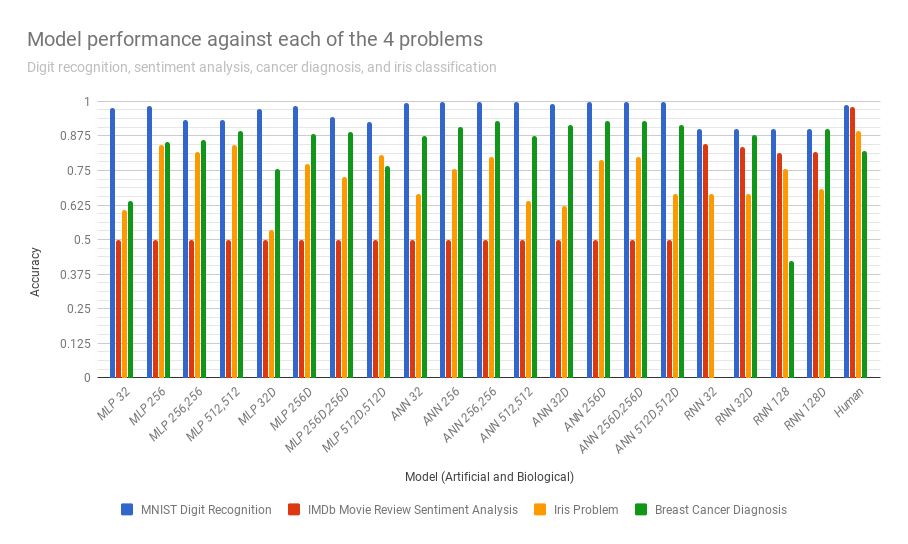
\includegraphics[width=\linewidth]{chart.png}
	\label{fig:chart0}
\end{figure}

\begin{figure}[H]
	\centering
	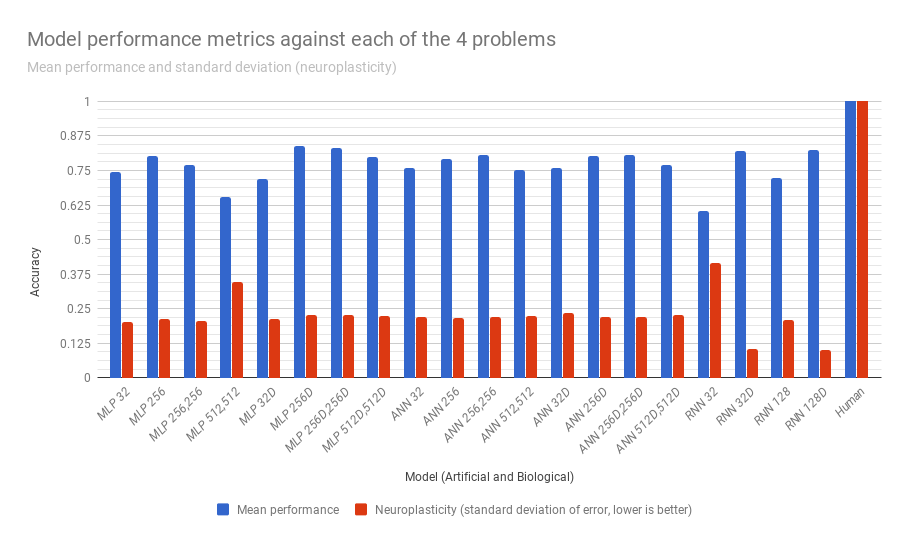
\includegraphics[width=\linewidth]{chart1.png}
	\label{fig:chart1}
\end{figure}

\begin{figure}[H]
	\centering
	\begin{subfigure}[b]{0.45\textwidth}
		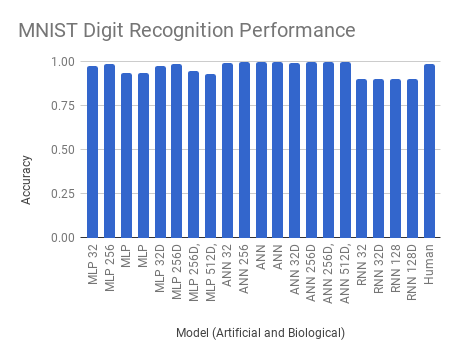
\includegraphics[width=\textwidth]{chart2.png}
	\end{subfigure}
	~
	\begin{subfigure}[b]{0.45\textwidth}
		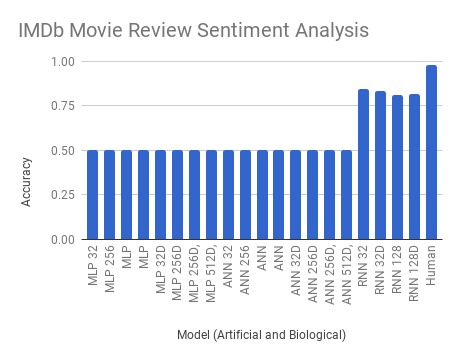
\includegraphics[width=\textwidth]{chart3.png}
	\end{subfigure}
	~
	\begin{subfigure}[b]{0.45\textwidth}
		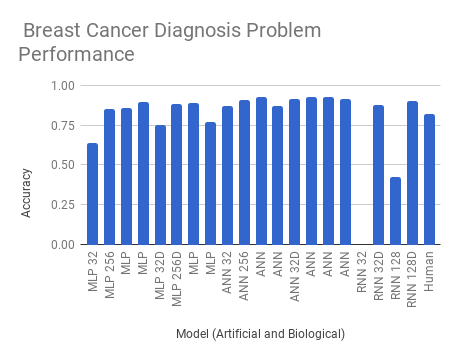
\includegraphics[width=\textwidth]{chart4.png}
	\end{subfigure}
~
	\begin{subfigure}[b]{0.45\textwidth}
		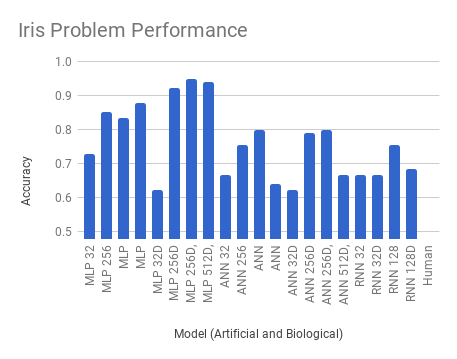
\includegraphics[width=\textwidth]{chart5.png}
	\end{subfigure}
\end{figure}


\section{Discussion}

The Recurrent Neural Networks performed the best across all problem domains, out of the artificial models. Of the RNNs, the most complex RNN with 1 hidden layer with 128 neurons and 20\% dropout performed the best, with an error standard deviation of 10.2\%, the lowest across all artificial models, and the third highest mean performance. The RNNs were heavily advantaged in the sentiment analysis problem, as they were the only models capable of building meaningful relationships about the data as it was sequential. None of the other models converged on the sentiment analysis problem, as they recieved the data as a single blob without word boundaries and with data scattered across the input layer without any format that remained constant for each step in the process of stochastic gradient descent. As a result, the accuracy on the sentiment analysis problem for all MLP and ANN models was equivalent to random guesswork over the 25000 test reviews supplied to the program; such that the accuracy was $\frac{1}{|C|} = \frac{1}{2} = 0.5$ where $C$ is a set of valid output classes (in this instance a set of two classes --- positive and negative sentiment).

Despite RNNs having the advantage in the natural language parsing problem domain, RNNs did not have time to fully converge in the MNIST digit recognition problem. Even when MNIST images were downsampled to a ninth of the size specifically for the MNIST-RNN test combination, each of the 8 epochs took an average of 20 minutes, as opposed to an average of 3.630 seconds in all of the ANN and MLP models. In fact, many of the more optimised ANN models (primarily those with 20\% dropout) began to diverge in under a minute, becoming so overfit to the training data that they lost accuracy on the test set. This is due to both the computational complexity of evaluating the data flow of an RNN relative to that of an ANN, and as there were thousands of times more trainable parameters subject to the stochastic gradient descent algorithm in RNNs as in the ANNs and MLPs (to illustrate, the smallest ANN had 59 trainable parameters, whereas the largest RNN had 233223 trainable parameters). ANNs were much faster to train (in one test run, the MLP 512D,512D achieved 99.41\% test accuracy after 3.640 seconds of training) and performed much better on non-sequential data, but entirely failed to converge on the sentiment analysis problem.

The high-end MLP and ANN models with dropout (MLP 512D,512D and ANN 512D,512D) reached extremely high accuracy on the MNIST digit recognition problem; the MLP achieved 99.71\% accuracy, a mere 0.06\% behind the world record (\cite{ciregan2012multi}), despite being one of the simpler models and requiring under a minute to complete 20 training epochs, using hardware acceleration on a consumer-grade GPU.

There was one test which failed entirely --- the RNN 32 against the cancer diagnosis problem. For some unknown reason the network failed to learn from the data entirely and persistently resulted in an accuracy of 0, although the RNN 32D which differed only in having 20\% dropout, achieved 87.67\% accuracy on the same problem. This error is likely due to a problem with the primary dependency Keras (see \textit{Appendix I}) or the way in which the programs used interface with it, as the RNN 32D and RNN 128 were both unaffected despite sharing the same code, aside from runtime parameters specifying the nature of the hidden layers.

Due to time constraints, it was not possible to fix the aforementioned error with the RNN 32 model, or to conduct experiments using support vector machines or people. However, this experimentation will be conducted before this report is submitted to the regional science fair competition and this report will be revised to incorporate new findings.


\section{Conclusion}

Overall, it is clear that Recurrent Neural Networks are the future of machine learning. Even if they don't necessarily use the LSTM neuron model used in this experiment, the way in which they are able to interpret sequential data makes them much more valuable across differing problem domains. They are also much more closely modelled to the human brain, which is and has been the blueprint for machine learning models since the inception of the field early last century, and is the source of inspiration for many of the successful model architectures within the field, from perceptrons to nonbinary LSTM neurons capable of drawing meaningful relationships in a series of sequential data.

However, the human brain performed the best in this experiment. Whilst many of the artificial models surpassed human ability in one or two models, no single artificial model surpassed the human brain in every task, despite the tasks being relatively simple for a neural network to solve (with the exception of the sentiment analysis problem). Despite having less training time on the cancer diagnosis and iris classification problems, the human brain was still the most neuroplastic across all of the problem domains.

All in all, this experiment has shown that state-of-the-art artificial intelligence techniques, despite having superhuman results in very narrow problem domains, are a ways off true general intelligence. The human brain still has 7 orders of magnitude more neurons than the most expansive of the models utilised in this experiment (1024 neurons compared to 100 billion, per \cite{herculano2009human}), and has mechanisms at play so complex that researchers have struggled even to fully simulate the brain of the C. Elegans, a transparent worm with only 959 neurons, whose connectome has been fully mapped for decades (\cite{wormwiring2012}). At the current point in time, neither the software to supervise the training of an AGI nor the hardware to implement the data flow of the network (let alone the training) exists, and will not for many decades at the current rate of progress.

\section{Appendices}

\subsection{Appendix I: Implementation Details}

The Python 3 source code files for all of the aforementioned artificial models are available online through the Git repository hosted at following URL: https://github.com/Tobsta/ScienceFair

All of the deep learning models tested were implemented in the Python 3 programming language, using the Keras machine learning library with a TensorFlow backend. It was decided to use a stable machine learning framework such as Keras to create easily reproducible results and to make it much easier to verify that the programs used in the experiment did not have any flaws undermining the validity of the experiment.

\twocolumn
\subsection{Glossary}
\begin{description}
\item[Activation function:] An activation/learning function is used to transform the output value of neurons to adapt the rate at which they learn.

\item[Artificial General Intelligence (AGI):] An AGI is an intelligent agent capable of learning to accomplish many general tasks at least as well as a human, as opposed to specialising in a particular task. At this stage, AGIs are mostly a topic of science fiction and radical speculation; however many experts believe that general intelligence is mere decades away. In a survey of prominent AI researchers, the median estimation for when there is a 50\% chance of AGIs having been developed was 100 years from 2016 (\cite{grace2017will}).

\item[Artificial Neural Network (ANN):] An interconnected network of artificial (ie. simulated) neurons that receive signals (in the form of binary or floating point numbers) as input, which pass through the connections between nodes in the network toward the output layer of neurons which emits a computed result. Simple ANNs typically contain an input layer, one or more hidden layers, and an output layer.

\item[Classification problem:] A classification problem is a type of machine learning problem in which a model is trained to classify data according to a few predefined classes. Examples include Optical Character Recognition and Computer Vision problems; the most common of which is handwritten digit recognition.

\item[Convolutional Neural Network (CNN):] A neural network in which some layers are not composed of artificial perceptrons.

\item[Cost function:] The cost function estimates the accuracy (error frequency) of a model; lower is better.

\item[Dropout:] Dropout is a technique to avoid overfitting in ANNs. It works by randomly removing a constant percentage (configurable as a hyper-parameter, defaulting to 20\% in this experiment) of nodes from a hidden layer in a neural network (\cite{dropout14}), which decreases the level of fine-tuning and makes computations by a model more generalised, with the additional benefit of making the model less computationally expensive to operate further into the training process.

\item[Feed-Forward ANN:] Feed-forward ANNs are a class of ANN which have distinct layers of neurons whose signals are only fed forward. This significantly reduces the complexity of neural networks, and means that the neural network is not capable of retaining information.

\item[Hidden Layer:] Hidden layers are layers of perceptrons in an ANN that do not directly deal with input or output, but instead perform highly complex logic through their unique combinations of neural connections (weights) and activation thresholds (biases).

\item[Hyper-parameter:] A hyper-parameter is a global parameter in an artificial model that is pre-selected by the model designer and which dictates how the model will be organised or how it will train. The number of neurons in a hidden layer and the learning rate are both examples of hyper-parameters.

\item[Input Layer:] The input layer of an ANN is the layer which doesn't take input from the previous layer, but rather from a sample in a dataset specific to the problem domain the ANN is being trained for.

\item[K-Means:] K-Means is a clustering algorithm, which attempts to find groups/clusters in a dataset with a known amount of classifications by recursively estimating the centre points (centroids) of each cluster.

\item[Learning function:] See \textit{Activation Function}

\item[Learning rate:] The learning rate is a hyper-parameter that is used as the maximum deviance random permutations made during the process of stochastic gradient descent may be. A higher learning rate means the model will train faster, but it also means it may not converge as well, unless the learning rate is exponentially decreased each epoch to make it more sensitive to fine-tuning.

\item[Long Short-Term Memory (LSTM):] LSTMs are a type of artificial neuron which are used in Recurrent Neural Networks (RNNs), which are designed to retain information for sequence processing.

\item[Machine Learning:] Machine learning is a subfield of computer science that deals with artificial intelligence, pattern recognition and the creation of inference engines.

\item[Neuroplasticity:] The ability of a brain or machine learning model to adapt to fit different problem domains without modifying the overall structure (i.e. by changing only the synapse connections and activation thresholds for neurons, and not the underlying algorithms).

\item[One-Hot Encoding:] One-hot encoding is the process of converting a class ID to an array of numbers equal to the number of classes, populated with zeros, aside from the number at the index of the class ID, which is a one. To illustrate, the classes "Cat", "Dog", and "Horse" could be represented as [1,0,0], [0,1,0], and [0,0,1] with one-hot encoding. One-hot encoding is much easier for an ANN to work with when operating on class-based data, especially in an output layer of a classification model (see softmax).

\item[Output Layer:] The output layer of an ANN is the layer which calculates the final result. In classification problems, each neuron in the output layer will typically map to a sample class. The result of the output layer is then compared to the one-hot encoded class of the sample in the cost function to determine the error rate.

\item[Overfitting:] If a model is overfit, it is so fine-tuned to operating on its training dataset that it performs poorly during validation and testing.

\item[Perceptron:] A perceptron is a common, but outdated, artificial model of a neuron which has a binary output as opposed to a floating-point one. This means that they are harder to train, as a small change in inputs creates a much larger change in output.

\item[Recurrent Neural Network (RNN):] An RNN is a neural network which runs recursively on a sequence of data, using previous inferences as input in addition to the chunks of the sequence data. RNNs are used for speech recognition, text classification (such as sentiment analysis) and many other problem domains in which the data is sequential and the length is variable; although RNNs can also be trained to work as less efficient ANNs with fixed vector size inputs and outputs.

\item[Regression problem:] A regression problem is a style of problem where a model is trained to find the relationship between input and output data. One example of a regression problem is estimating the selling price of a house given data on it (number of bedrooms, size of the block, etc.)	

\item[ReLU] ReLUs (Rectified Linear Units) are a simple activation (learning) function that returns the input or 0, whichever is greater.

\item[RMSprop] RMSprop is a learning algorithm (not to be confused with a learning/activation function) similar to stochastic gradient descent, except instead of specifying a learning rate hyper-parameter the learning rate is adjusted given the gradient of each trainable parameter of the model. This means that the model is immune to both falling into a local minimum and plateauing during training, and to being so insensitive to a steep gradient that it diverges away from the global maximum.

\item[Sigmoid function:] The sigmoid function is a learning function that creates an S-shaped curve.

\label{itm:SGD}
\item[Stochastic Gradient Descent (SGD):] A method of minimising the error function of a neural network model (or other machine learning model) given multivariate input, in which the the input parameters are viewed as axes on an n-dimensional graph with the cost function as the Y-axis. SGD attempts to find the global minimum of the cost function without calculating it for every possible combination of parameters by rolling the ball (vector representing the weights and biases of the neural network) down the hill (this analogy only really works with 2 parameters as the X and Z axes and the cost function as the Y axis, but it can be expanded to work with n dimensions.) Local minimums are avoided by the learning rate hyper-parameter, indicative of the length of the step taken (ideally toward the global minimum) in each iteration of the SGD algorithm. The direction gradient toward the local minimum is estimated by calculating the partial derivative of the cost function with respect to each parameter, and determining which parameter, plus-minus the learning rate hyper-parameter, has the lowest result of the cost function.

\item[Softmax:] Softmax is an activation (learning) function that scales all outputs from a layer from 0 to 1, such that the sum of all outputs is 1. It is typically used for the output layer of a classification neural network, as a kind of floating-point one-hot encoding method.

\item[Support Vector Machine (SVM):] SVMs are an older method of machine learning which uses mathematically and not biologically inspired linear and non-linear regression algorithms to classify numerical data into distinct classifications.
\end{description}
\onecolumn

\printbibliography

\end{document}          
